\chapter{Materiais e Métodos}
\label{ch:4_MateriaisMetodos}
Nesse capítulo são apresentados as ferramentas computacionais que foram utilizadas para o desenvolvimento desse trabalho, o caso de estudo definido para a aplicação dos AGs propostos anteriormente e a metodologia utilizada para a execução dos experimentos. 

\section{Ferramentas Computacionais}
\label{ch:4_FerramentasComputacionais}
Para obter os indicadores técnicos e econômicos para a avaliação de uma estratégia de produção é necessário o uso de algumas ferramentas computacionais como o IMEX\footnote{Mais informações em: https://www.cmgl.ca/imex} , utilizado para a simulação de campo de petróleo, e o MERO\footnote{Mais informações em: https://goo.gl/J7WD22} , que interpreta os resultados da simulação e obtém os indicadores econômicos e de poços. Para a implementação dos AGs e dos operadores de busca foi utilizado como base o \textit{framework} JMetal\footnote{Mais informações em: http://jmetal.sourceforge.net/}  e, por fim, para comparação dos resultados obtidos pelos AGs foi utilizado a ferramenta de otimização CMOST\footnote{Mais informações em: https://www.cmgl.ca/cmost-ai} . Os tópicos a seguir apresentam com mais detalhes a ferramentas citadas.

\subsection{IMEX}
\label{ch:4_IMEX}
O desenvolvimento deste trabalho exigiu o uso de um simulador comercial de reservatórios para que a qualidade geral das estratégias de produção propostas e seus efeitos no comportamento do reservatório ao longo do tempo pudessem ser avaliados. Sendo assim, foi utilizado aqui o software IMEX, na versão 2012.1, que é um simulador \textit{black oil} desenvolvido pela CMG. 

\subsection{MERO}
\label{ch:4_MERO}
Além do simulador IMEX, também foi utilizado neste trabalho o software MERO, desenvolvido pelo UNISIM. Este software é formado por uma série de módulos auxiliares responsáveis pela interface entre a implementação das meta-heurísticas que foram feitas neste trabalho e o simulador IMEX. Além disso, o MERO também possui módulos que complementam os resultados retornados pelo IMEX, sendo capaz de, a partir dos resultados da simulação do campo de petróleo para uma dada estratégia de produção, calcular o VPL total que será obtido ao final do período de concessão, retornando este valor para o algoritmo de otimização implementado. Quatro módulos do MERO foram utilizados neste trabalho:

\subsubsection{Módulo de Geração de Eventos}
\label{ch:4_ModuloGeracaoEventos}
Este módulo é responsável por gerar um arquivo contendo dados de eventos relacionados à estratégia de produção como, por exemplo, a definição de datas para a instalação da plataforma, para o início e abandono das operações no campo de petróleo, para abertura e fechamento dos poços e os dados de localização, tipo e direção destes poços. Para utilizar esta ferramenta é necessário definir um arquivo de entrada listando os eventos da estratégia de produção. Este arquivo de eventos é utilizado posteriormente para a criação dos arquivos de simulação e cálculo dos indicadores econômicos da estratégia de produção.

\subsubsection{Módulo de Geração de Estratégia de Produção}
\label{ch:4_ModuloGeracaoEstrategiProducao}
Este módulo é responsável por criar os arquivos de simulação que serão enviados para o software de simulação IMEX. Para que tal ferramenta funcione adequadamente é necessário indicar um arquivo com os eventos da estratégia de produção, um arquivo contendo informações econômicas, como impostos e valores do mercado, e um arquivo com informações do reservatório de petróleo cujo comportamento deverá ser simulado. 

\subsubsection{Módulo de Cálculo da Função de Desempenho}
\label{ch:4_ModuloCalculoFuncaoDesempenho}
Este módulo realiza o cálculo dos indicadores econômicos e técnicos relacionados à simulação da estratégia de produção. Para tal é necessário indicar, para a ferramenta, o arquivo de simulação, o arquivo contendo os eventos da estratégia de produção e o arquivo com os dados econômicos.

\subsubsection{Módulo de Composição de Fluxos de Trabalho }
\label{ch:4_ModuloComposicaoFluxosTrabalho}
Este módulo permite criar um fluxo de trabalho com as ferramentas do Mero, sendo possível indicar, sequencialmente, quais ferramentas deseja-se utilizar e estabelecer os dados necessários para cada ferramenta em um arquivo de entrada pré-definido. Neste trabalho, esta ferramenta foi utilizada para executar sequencialmente os módulos de Geração de Eventos, Geração da Estratégia de Produção e de Cálculo da Função de Desempenho.

\subsection{JMetal}
\label{ch:4_JMetal}
JMetal é um \textit{framework} e uma biblioteca de código livre, escrito em Java, que pode ser utilizado para resolver problemas de otimização multiobjetivo com meta-heurísticas \cite{Durillo2011}. Apesar do seu foco em problemas multiobjetivo, esta biblioteca também fornece algoritmos para problemas de objetivo único, como o que será tratado neste trabalho. Foi utilizada aqui a versão 5.1 do JMetal, que foi revisada e simplificada para facilitar a implementação de algoritmos para solução de diversos problemas \cite{Nebro2015}. Especificamente no contexto deste trabalho, em um primeiro momento foi utilizada a implementação das versões clássicas do AG e dos operadores que esse \textit{framework} oferece. Posteriormente a estrutura que o JMetal oferece foi utilizada como base para implementação das versões modificadas do algoritmo genético e dos operadores de recombinação e mutação específicos para o problema de DEP, apresentados no capítulo anterior. 

\subsection{CMOST}
\label{ch:4_CMOST}
Também desenvolvido pela CMG, o CMOST é uma ferramenta para resolver problemas de otimização que foi utilizada neste trabalho para que os resultados obtidos pelos algoritmos implementados pudessem ser comparados com os obtidos por uma ferramenta comercial. A versão utilizada nesse trabalho foi a versão 2012.10.

Essa ferramenta utiliza um método proprietário para realizar o processo de otimização. Tal método é dominando como DECE (\textit{Designed Exploration and Controlled Evolution}) e, em resumo, o processo é dividido em duas etapas (i) exploração projetada e (ii) evolução controlada \cite{CMG2012}. Durante a primeira etapa, o objetivo é explorar o espaço de busca de uma maneira aleatória, utilizando técnicas de Design Experimental e Busca Tabu, para adquirir um conjunto de dados dos valores de parâmetros e criar um conjunto representativo de simulações. A segunda etapa análises estatísticas são realizadas sobre o conjunto de dados levantado durante a etapa anterior para definir se há chances de melhorar a qualidade das soluções ao impedir que alguns valores dos parâmetros sejam escolhidos. Afim de minimizar as chances de cair em uma solução de ótimo local, o DECE verifica de tempos em tempos os valores marcados como rejeitados para garantir que tais rejeições ainda são válidas, caso não seja os valores são considerados novamente para o processo de otimização.

Além do DECE, o CMOST permite utilizar outros algoritmos de otimização tal qual o Hipercubo Latino, Enxame de Partículas, Busca por Força Bruta e Busca Aleatória. Vale ressaltar que nesse trabalho o CMOST foi configurado para utilizar o algoritmo proprietário DECE.

\section{Caso de Estudo}
\label{ch:4_CasoEstudo}
Os experimentos realizados nesse trabalho utilizaram um modelo de reservatório cedido pelo grupo UNISIM, correspondente a um campo sintético baseado no campo de Namorado, localizado no Rio de Janeiro. O modelo em questão foi construído com base nos dados obtidos através de quatro poços exploratórios verticais que foram perfurados no campo e da sísmica disponível para a área \cite{Silva2016}, resultando em um campo sintético com 8568 blocos, sendo 5174 blocos ativos. A Figura 5 apresenta as visões em 2D e 3D do modelo utilizado.

\begin{figure}[htb]

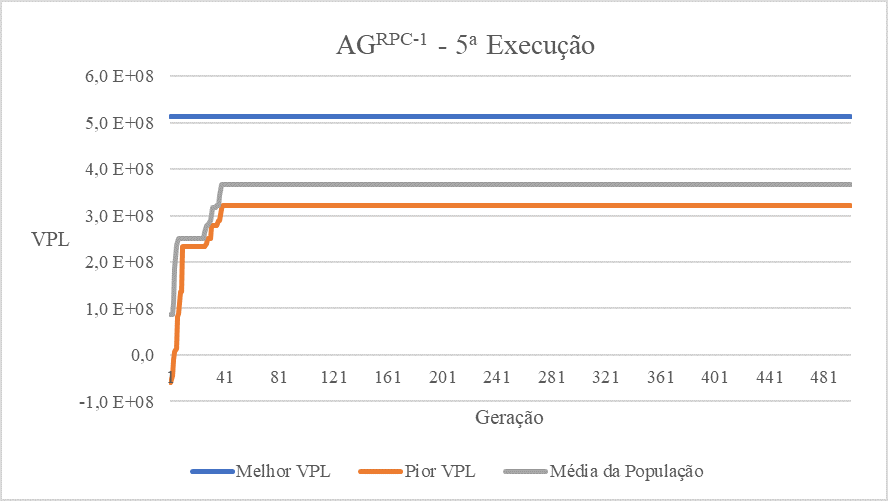
\includegraphics[scale=0.7]{5.png}

\caption{Visualização em 2D (a) e 3D (b) do modelo de reservatório sintético baseado no campo de Namorado.}

\end{figure}

Os parâmetros do problema de DEP a ser otimizado para esse campo sintético, utilizando os algoritmos desenvolvidos nesse trabalho, foi definido em conjunto com os engenheiros do grupo UNISIM. Segundo \citeonline{PedrosoJunior1999}, o posicionamento dos poços de uma estratégia de produção é um dos principais parâmetros a ser definido para o sistema de produção, sendo assim, o problema definido aqui consiste em otimizar a posição de 18 poços de uma estratégia de produção, no qual dez desses poços são do tipo produtor e oito poços do tipo injetor. Cada um desses poços é do tipo horizontal e ocupa três blocos do modelo do reservatório. A Tabela \ref{table:params} apresenta os parâmetros utilizados para a os cálculos dos indicadores econômicos durante a simulação de campo de petróleo.

\begin{table}[H]
\centering

\caption{Parâmetros econômicos utilizados para a simulação de campo de petróleo.}
\label{table:params}
 \begin{tabular}{|c|c|c|} 
\hline
 \multicolumn{2}{|c|}{\textbf{Parâmetro}} & \textbf{Valor} \\ \hline
 \multirow{3}{*}{\textbf{Custos de Produção e Injeção}} & Produção de Óleo (US\$/ m3) & $62,90$ \\
 & Produção de Água (US\$/ m3) & $6,29$ \\ 
 & Injeção de Água (US\$/ m3) & $6,29$\\ \hline
 \multirow{3}{*}{\textbf{Impostos}} & PIS/Cofins (\%) & $0,09$ \\
 & Imposto de Renda / Contribuição Social(\%) & $0,34$ \\
 & Royalty (\%) & 0,10 \\ \hline
 \multirow{3}{*}{\textbf{Valores de Mercado}} & Taxa de Atratividade(\%) & 0,09 \\
 & Preço do Petróleo (US\$/ m3) & 314,50 \\
 & Custo do Poço (Milhões de US\$)& 2,34 \\ \hline
 
\end{tabular}
\end{table}

\section{Metodologia Experimental}
\label{ch:4_MetodologiaExperimental}
Como foi apresentado no Tópico 2.2, é preciso definir uma série de operadores e parâmetros para o bom funcionamento da meta-heurística. Em relação ao algoritmo genético são três os operadores que precisam ser definidos: o operador de seleção, o operador de recombinação e o operador de mutação, além desses, aqui também foi utilizado um operador de busca local para refinar as soluções do AG. Quanto aos parâmetros é preciso definir a quantidade máxima de avaliações da função objetivo, o tamanho da população, a probabilidade de ocorrer uma recombinação entre as soluções da população e a probabilidade de ocorrer uma mutação as soluções geradas. Vale ressaltar que a quantidade máxima de avaliações da função objetivo foi definido como critério de parada para todos os algoritmos executados, essa escolha foi feita para tornar mais justa a comparação entre os resultados obtidos, uma vez que os algoritmos possuem a mesma quantidade de iterações para encontrar a melhor solução possível para o problema.

A cada experimento realizado nesse trabalho procurou-se explorar uma versão do AG proposta no no Tópico 3.3 com um conjunto de operadores e parâmetros. Dado o caráter estocástico do algoritmo, a cada experimento o AG estudado foi executado dez vezes, então, a partir dos resultados foram calculados a média do melhor VPL encontrado em cada execução, o desvio padrão e o tempo médio gasto para que cada execução fosse concluída. Para constatar que a diferença entre os resultados obtidos pelos algoritmos estudados são estatisticamente significativas, o teste estatístico não-paramétrico de Mann-Whitney-Wilcoxon \cite{Corder2014} foi aplicado considerando-se um limiar de 5\%. Em outras palavras, caso o resultado do teste (denominado p-\textit{value}) apresente um valor maior que o limiar de 5\%, os dois conjuntos que foram aplicados ao teste não diferem entre si. Sendo assim, tanto faz utilizar um algoritmo ou outro. 

Ao todo foram realizados sete experimentos separados em duas etapas, a principal diferença entre as etapas está no número total de avaliações da função objetivo realizado pelos algoritmos e o uso do operador de busca local em conjunto com o AG. Tal operador foi considerado somente na segunda etapa. Além dos AGs, foram executados o CMOST e uma Busca Aleatória para fim de comparação, vale ressaltar ambos utilizaram o mesmo critério de parada estabelecido para os AGs. Os próximos tópicos apresentam mais detalhes das configurações utilizadas em cada experimento das duas etapas.

\subsection{Etapa 1}
\label{ch:4_Etapa1}
O foco dessa primeira etapa foi explorar o uso dos algoritmos genéticos sem o operador de busca local. Para todos os experimentos dessa etapa foi estabelecido um máximo de 500 avaliações da função objetivo. Quando se trata de meta-heurísticas populacionais, é comum que o número máximo de avaliações da função objetivo seja muito maior que o valor e estabelecido. Facilmente encontra-se trabalhos onde tal valor chega a $10^6$ \cite{Elsayed2016,Tangherloni2017,Kumar2017,Zamuda2017}. Outro exemplo disso são os próprios valores pré-definidos pelo JMetal, que nesse caso é de 25.000 avaliações. No entanto, adotar um número tão alto nesse trabalho tornaria inviável o uso dos algoritmos genéticos para a resolução do problema estudado, dado a dificuldade de se avaliar uma estratégia de produção, principalmente em relação ao tempo computacional necessário para concluir uma simulação de campo de petróleo. Por esse motivo, um valor consideravelmente baixo foi definido para esse parâmetro. 

Outro parâmetro que não variou no decorrer dos experimentos foi a probabilidade de recombinação. Como foi discutido no Capítulo 2.1, o operador de recombinação apresenta um papel importante durante a execução do algoritmo genético. Sendo assim, optou-se por atribuir uma probabilidade de 100\% para a execução desse operador. Dessa forma garante-se que, para cada par de indivíduos selecionados para a recombinação, um novo indivíduo será gerado pelo operador. Quanto aos demais operadores e parâmetros, alteraçõe foram realizadas no decorrer dos experimentos. A Tabela \ref{table:con01} apresenta a configuração utilizada para o Experimento 1 dessa primeira etapa.

\begin{table}[H]
\centering
\caption{Versões do AG e os operadores de busca utilizados em cada experimento}
\label{table:con01}
\begin{tabular}{|p{6cm}|p{9cm}|}
\hline
\multicolumn{2}{|c|}{\textbf{Experimento 1}} \\ \hline
{\textbf{Algoritmo}} & AG Geracional Clássico ($AG^{GC-1}$) e AG de Regime Permanente Clássico ($AG^{RPC-1}$) \\ \hline
\textbf{Operador de seleção} & Torneio Binário \\ \hline
\textbf{Operador de Recombinação} & Recombinação Uniforme \\  \hline
\textbf{Operador de Mutação} & Pontual \\ \hline
\textbf{Número Total de Avaliações} & 500 \\ \hline
\textbf{Tamanho da População} & 10 \\ \hline
\textbf{Probabilidade de Recombinação (\%)} & 100 \\ \hline
\textbf{Probabilidade de Mutação (\%)} & 1 \\ \hline
\end{tabular}
\end{table}

Nesse primeiro experimento foi utilizado tanto a versão clássica do AG (Geracional e de Regime Permanente) quanto operadores clássicos recombinação e mutação. Aqui o intuito foi observar como o AG puro se comporta para resolver o problema estudado. Vale ressaltar aqui o valor atribuído para a probabilidade  de mutação. Foi estabelecido o valor de 1\% seguindo a recomendação da literatura de manter baixa tal probabilidade. Esse valor de 1\% também corresponde ao valor padrão definido para os operadores encontrados no \textit{JMetal}. O tamanho da população também foi relativamente baixo para garantir que o número de gerações fosse maior. Uma vez que o AG Geracional realiza mais de uma avaliação da função objetivo a cada iteração.

Como é possível observar pela Tabela \ref{table:con02}, grande parte das configurações estabelecidas no Experimento 1 foram mantidas para o Experimento 2,

\begin{table}[H]
\centering
\caption{Versões do AG e os operadores de busca utilizados em cada experimento}
\label{table:con02}
\begin{tabular}{|p{6cm}|p{9cm}|}
\hline
\multicolumn{2}{|c|}{\textbf{Experimento 2}} \\ \hline
{\textbf{Algoritmo}} & AG Geracional Clássico ($AG^{GC-2}$) e AG de Regime Permanente Clássico ($AG^{RPC-2}$) \\ \hline
\textbf{Operador de seleção} & Torneio Binário \\ \hline
\textbf{Operador de Recombinação} & Gera os novos indivíduos (filhos) aleatoriamente dentro da região delimitada pelas coordenadas dos dois pais \\  \hline
\textbf{Operador de Mutação} & Pontual \\ \hline
\textbf{Número Total de Avaliações} & 500 \\ \hline
\textbf{Tamanho da População} & 10 \\ \hline
\textbf{Probabilidade de Recombinação (\%)} & 100 \\ \hline
\textbf{Probabilidade de Mutação (\%)} & 1 \\ \hline
\end{tabular}
\end{table}

A principal mudança realizada nesse experimento foi em relação ao operador de recombinação, aqui sai o operador de  Recombinação Uniforme e entra o operador proposto no Tópico 3.5 que atribui uma posição ao poços da solução gerada a partir de uma área delimitada pela posição dos poços das soluções pais.

Para o terceiro experimento foi alterado o tamanho da população. Observou-se que um  aumento da população  poderia levar a um ganho no desempenho do AGs uma vez que esse algoritmo utiliza a população como um repertório para buscar novas soluções. Com um repertório maior, mais chances de haver uma diversidade maior de soluções. Uma característica importante para o bom funcionamento de uma meta-heurística populacional. Como é possível notar pela Tabela \ref{table:con03} os outros operadores e atributos foram mantidos.
\begin{table}[H]
\centering
\caption{Versões do AG e os operadores de busca utilizados em cada experimento}
\label{table:con03}
\begin{tabular}{|p{6cm}|p{9cm}|}
\hline

\multicolumn{2}{|c|}{\textbf{Experimento 3}} \\ \hline
\textbf{Algoritmo} & AG Geracional Clássico ($AG^{GC-3}$) e AG de Regime Permanente Clássico ($AG^{RPC-3}$) \\ \hline
\textbf{Operador de seleção} & Torneio Binário \\ \hline
\textbf{Operador de Recombinação} & Gera os novos indivíduos (filhos) aleatoriamente dentro da região delimitada pelas coordenadas dos dois pais \\  \hline
\textbf{Operador de Mutação} & Pontual \\ \hline
\textbf{Número Total de Avaliações} & 500 \\ \hline
\textbf{Tamanho da População} & 100 \\ \hline
\textbf{Probabilidade de Recombinação (\%)} & 100 \\ \hline
\textbf{Probabilidade de Mutação (\%)} & 1 \\ \hline
 \end{tabular}
\end{table}

Ao observar os resultados obtidos pelos três experimentos realizados até então, constatou-se que o AG de Regime Permanente teve um desempenho superior ao AG Geracional. Tendo isso como base, a variação de Regime Permanente foi a escolhida para a criação da versão modificada proposta no Tópico 3.3.2. Essa versão do algoritmo foi a utilizada pelo quarto experimento realizado durante a Etapa 1. Além disso, aqui também foi utilizado o operador de mutação proposto no tópico 3.6. A configuração adotada nesse experimento pode ser vista na Tabela \ref{table:con04}.

\begin{table}[H]
\centering
\caption{Versões do AG e os operadores de busca utilizados em cada experimento}
\label{table:con04}
\begin{tabular}{|p{6cm}|p{9cm}|}
\hline
 
 \multicolumn{2}{|c|}{\textbf{Experimento 4}} \\ \hline
\textbf{Algoritmo} & AG Primeira Modificação do AG de Regime Permanente ($AG^{RPM}$) \\ \hline
\textbf{Operador de seleção} & Torneio Binário \\ \hline
\textbf{Operador de Recombinação} & Gera os novos indivíduos (filhos) aleatoriamente dentro da região delimitada pelas coordenadas dos dois pais \\  \hline
\textbf{Operador de Mutação} & Altera aleatoriamente a posição dos poços de acordo com o IEP do poço \\ \hline
\textbf{Número Total de Avaliações} & 500 \\ \hline
\textbf{Tamanho da População} & 100 \\ \hline
\textbf{Probabilidade de Recombinação (\%)} & 100 \\ \hline
\end{tabular}
\end{table}

É possível notar a inexistência do valor para a probabilidade de mutação nesse experimento. Isso ocorre porque a partir desse experimento é utilizado o operador de mutação proposto no Capítulo 3.4, sendo que para tal operador não é necessário atribuir um valor de probabilidade para ser executado uma vez que esse operador só é executado caso a solução candidata venha a ser descartada da população após sua avaliação.

Por fim, a Tabela \ref{table:con05} apresenta a configuração adotada para o quinto experimento da Etapa 1. 

\begin{table}[H]
\centering
\caption{Versões do AG e os operadores de busca utilizados em cada experimento}
\label{table:con05}
\begin{tabular}{|p{6cm}|p{9cm}|}
\hline
 
 \multicolumn{2}{|c|}{\textbf{Experimento 5}} \\ \hline
\textbf{Algoritmo} &AG de Regime Permanente com o Operador de Contagem de Ocorrências ($AG^{CO}$) \\ \hline
\textbf{Operador de seleção} & Torneio Binário \\ \hline
\textbf{Operador de Recombinação} & Gera os novos indivíduos (filhos) aleatoriamente dentro da região delimitada pelas coordenadas dos dois pais \\  \hline
\textbf{Operador de Mutação} & Altera aleatoriamente a posição dos poços de acordo com o IEP do poço \\ \hline
\textbf{Número Total de Avaliações} & 500 \\ \hline
\textbf{Tamanho da População} & 100 e 50 \\ \hline
\textbf{Probabilidade de Recombinação (\%)} & 100 \\ \hline
\end{tabular}
\end{table} 

Para o quinto experimento foi utilizado a segunda versão modificada do AG, proposta no Tópico 3.3.3. A principal característica dessa versão é o uso de um operador para contar a ocorrências dos valores do intervalo definido para cada uma das coordenadas para a localização dos poços. Para observar melhor o comportamento dessa versão do algoritmo foi estabelecido dois tamanho da população, como é possível notar pela tabela \ref{table:con05}. Para finalizar, vale ressaltar novamente que os algoritmos aqui executados foram tiveram seus resultados comparados com uma Busca Aleatória e o CMOST, ambos realizando um  máximo de 500 avaliações e sendo executados de vezes.

\subsection{Etapa 2}
\label{ch:4_Etapa2}
Para os experimentos da segunda etapa foi utilizado o AG que obteve o melhor desempenho durante a Etapa 1. Em conjunto com essa versão do AG foi utilizado as duas variações da Busca Local proposta no Tópico 3.7. Aqui também foi atribuído o máximo de 500 avaliações da função objetivo  para o AG, no entanto o número total de avaliações realizadas durante os experimentos dessa etapa é maior por conta do operador de busca local que realiza mais avaliações ao fim da execução do AG. Como será possível ver no Capítulo 5, tal operador precisou de cerca de 220 avaliações para concluir sua execução. Sendo assim, em média, o total foi de aproximadamente 720 avaliações. A configuração adotada para o Experimento 1 da Etapa 2 pode ser vista na Tabela \ref{table:con06}.

\begin{table}[H]
\centering
\caption{Versões do AG e os operadores de busca utilizados em cada experimento}
\label{table:con06}
\begin{tabular}{|p{6cm}|p{9cm}|}
\hline

\multicolumn{2}{|c|}{\textbf{Experimento 1}} \\ \hline
\textbf{Algoritmo} & Primeira versão modificada do AG de Regime Permanente  \\ \hline
\textbf{Operador de seleção} & Torneio Binário \\ \hline
\textbf{Operador de Recombinação} & Gera os novos indivíduos (filhos) aleatoriamente dentro da região delimitada pelas coordenadas dos dois pais \\  \hline
\textbf{Operador de Mutação} & Altera aleatoriamente a posição dos poços de acordo com o IEP do poço \\ \hline
\textbf{Operador de Busca Local} & Primeira versão do operador de Busca Local ($AG^{BL-1}$) \\ \hline
\textbf{Número Total de Avaliações} & 720 \\ \hline
\textbf{Tamanho da População} & 100 \\ \hline
\textbf{Probabilidade de Recombinação (\%)} & 100 \\ \hline
\end{tabular}
\end{table}

Por fim a Tabela \ref{table:con06} apresenta a configuração adotada para o segundo experimento da Etapa 2. A principal alteração é em relação ao operador de busca local, aqui foi utilizada a segunda proposta para tal operador que também foi apresentada no Tópico 3.7.

\begin{table}[H]
\centering
\caption{Versões do AG e os operadores de busca utilizados em cada experimento}
\label{table:con07}
\begin{tabular}{|p{6cm}|p{9cm}|}
\hline

\multicolumn{2}{|c|}{\textbf{Experimento 2}} \\ \hline
\textbf{Algoritmo} & Primeira versão modificada do AG de Regime Permanente \\ \hline
\textbf{Operador de seleção} & Torneio Binário \\ \hline
\textbf{Operador de Recombinação} & Gera os novos indivíduos (filhos) aleatoriamente dentro da região delimitada pelas coordenadas dos dois pais \\  \hline
\textbf{Operador de Mutação} & Altera aleatoriamente a posição dos poços de acordo com o IEP do poço \\ \hline
\textbf{Operador de Busca Local} & Segunda versão do operador de Busca Local ($AG^{BL-2}$) \\ \hline
\textbf{Número Total de Avaliações} & 680 \\ \hline
\textbf{Tamanho da População} & 100 \\ \hline
\textbf{Probabilidade de Recombinação (\%)} & 100 \\ \hline
\end{tabular}
\end{table}

Vale ressaltar que durante essa etapa o AG que obteve o melhor desempenho e o CMOST foram executados novamente, no entanto, com um número maior de avaliações da função objetivo para tornar mais justas as comparações realizadas. Tanto o AG (sem o operador de busca local) quanto o CMOST foram executados aqui realizando uma quantidade máxima de 730 avaliações da função objetivo. Por fim, a máquina utilizada para os testes possuía a seguinte configuração: 

\begin{itemize}
\item Sistema Operacional: Windows 10 Pro;
\item Processador: Intel Core i5-4590 de 3,3GHz;
\item Memória RAM: 8 GB de 800MHz;
\item Disco rígido: 500 GB de 7200 RPM;
\item Placa de Vídeo Integrada: Intel HD \textit{Graphics} 4000.
\end{itemize}

